\documentclass[../main/main.tex]{subfiles}

\newdate{date}{29}{04}{2020}

\begin{document}

\section{Lecture 15}
 \displaydate{date}. Compiled:  \today. Alice.
 

\subsubsection{Slide 227}

\begin{figure}[h!]
\centering
\includegraphics[page=10,width=0.9\textwidth]{../lessons/pdf_file/14_lesson.pdf}
\end{figure}

In the previous lesson we have addressed the problem of answering this apparently silly question of what is the color of the gold nanoclusters. To answer to this question which is not silly as one can think, we have experimentally measure the difference in the absorbance in a gold film and in a colloidal solution of gold nanoparticle with a low volumetric filling fraction \( \Phi  \). We have concluded that the major difference occurred in the visible or near infrared range, whereas in the near UV range the two absorption looks quite similar. This means that the dielectric properties which controls this absorption should be quite similar in that region, and should be quite different in the other region. We have concluded that the descreasing in the capability of absorbing phtons with arbitrary small energy in gold colloidal clusters stands from the quantum confinement, but we inferred this conclusion just considering a pure model of a particle in a box and the description of free electrons in metals which  is ok. But we would like to obtain general rules to describe the dielectric properties of a metallic nanoparticle as a function of size. So that we can go trough this ladder of sizes (i pallini crescenti in figura), going from the bulk gold film dump to the atom, and going trough different sizes. But not just solving the hamiltonian of the Schr$\ddot{o}$dinger equation for all those sizes (which becomes impractible as soon as the number of atoms increase). Atoms like gold possess a lot of electrons, so the quantum mechanical description of the entire set of electrons is a formidable task. We would like to follow a top down approach just to see how we can go from a bulk like description of the dielectric properties of the material to (in particular metal) down to nanosize. We will see how to do that with a size equation, which is a technique that we have already learned from the first lesson of this course. So let us see how we can obtain that.

\newpage
\subsubsection{Slide 228}

\begin{figure}[h!]
\centering
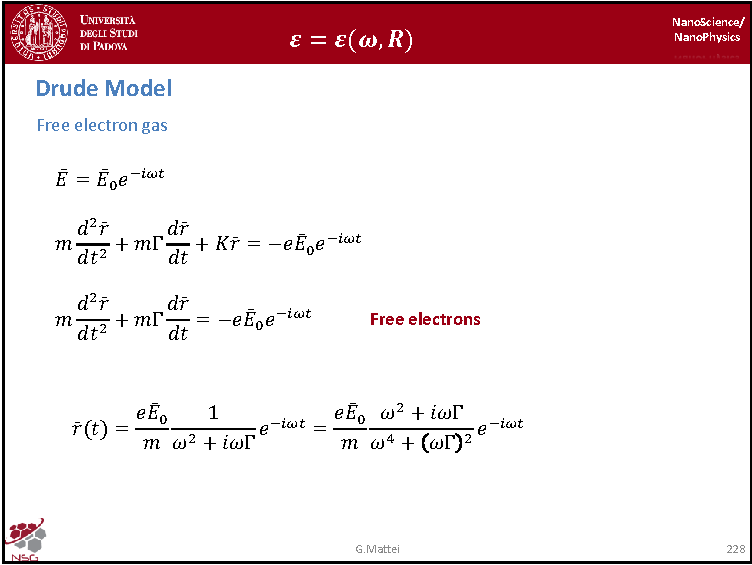
\includegraphics[page=1,width=0.9\textwidth]{../lessons/pdf_file/15_lesson.pdf}
\end{figure}

The first ingredient that we need is a dielectric of a bulk metal. You may remember from the solid state physics course, we obtained already this dielectric function in the so called Drude model approximation (which is a purely classical model, which describes electrons as freely moving in space) and we already discussed the limits of the Drude model in terms of the physical interpetation. But as you may remember, the equations which the Drude model produces looks exactly the same as the fully quantum mechanical description of the electrons motion in the metal at fully quantum mechanical level. So we will stay on the Drude model just to speed up the calculations.

You may remember that the major assumptions of the Drude model were the non-interacting electron approximation (so each electron is considered as independent) and the fact that the electrons do not interact also with the positive background, but just there is a mechanism of interaction which arises from the point-like interaction when electrons hit a positive core (like a sort of Brownian motion). Just to briefly recap the basic ingredient of the Drude model, if we send an electric field which is homogeneous across the entire volume of our metal, but it varies in time harmonically, the electrons behaves independently. So the equation of motion can be written as in (1), where there is the mass \( m \), the acceleration, the viscous term which arises from the interaction, or the balistic interaction, between the electrons and the positive corse. In principle, we could had a term which could take into account the elastic interaction of electrons with the cores, but since we are dealing with free electrons, we switch off totallyy this term \( k \va{r} \). Then we have the Lorentz force \( -e \va{E_0} e^{- i \omega t}  \), which is the external force in our system. So the equation is very simple and you now very well how to solv it. The trick is to find a solution in which the temporal evolution should be the same of the force field \( e^{- i \omega t}  \), so the homogeneous solution (that is when the right hand of the equation goes to zero) is nothing that (3). So \( \va{r } (t) \) is a constant times the harmonic evolution.

Just to briefly recall the meaning of the terms, the \( \Gamma  \) is nothing than the frequency at which electrons impinges on the positive ionic core. So this is an average number and it is the inverse of the relaxation time, which is the average time between two different interactions between electrons and the cores. So by substitution is straightforward to arrive at the expression (3) for the r coordinate as a function of time. This is an oscillating value, which is in phase with the pumping external field, and of course the amplitude of the oscillation is proportional to the amplitude of the pumping field. There is this frequency dependence of the amplitude.


\newpage
\subsubsection{Slide 229}

\begin{figure}[h!]
\centering
\includegraphics[page=2,width=0.9\textwidth]{../lessons/pdf_file/15_lesson.pdf}
\end{figure}

If we look at the collective behavior of all the electrons, each electron (since it is unbalanced with respect of the average position in the free electrons), it produces a dipole moment, which is:
\begin{equation*}
  \va{p} (t) \equiv - e \va{r} (t)
\end{equation*}
where \( e \) is the oscillating charge and \( \va{r} \) is the relative coordinate with respect to the equilibrium position (the original position).
So this induced dipole moment per electron is in phase with the field and it oscillates with an amplitude that is in the opposite side of course: when the field goes up the dipole moment goes down because of the minus sign in front of the expression.

We can define a polarization of our system, that is if we have a concentration of electrons \( n \) (\( n \) electrons per unit volume), times the induced dipoles (as all the electrons behave similarly). We can write the dipole moment as \( \varepsilon _0 \alpha \va{E} \) (where \( \alpha  \) is the polarizability) for electric material. In the end, we can rewrite this simple equation with a constitutive equation relating the polarization with the external field trough the concept of linear susceptibility. This is the first order of the linear susceptibility.

As far as the displacement field, which is related to the electric field by the multiplication for the \( \varepsilon _0 \varepsilon  \) (were \( \varepsilon  \) is the relative dielectric function in our system), we can rewrite this equation introducing the polarization. So the displacement takes into account the polarization induced in the material \(\va{P} \) and so we can rewrite the polarization with the previous expression. Then we can factorize the term arriving at a simple expression:
\begin{equation*}
  \va{D} = \varepsilon _0 (1 + \chi ) \va{E}
\end{equation*}
in which we have the linear suscpetibility and the relative dielectric function which is \( \varepsilon  \) :
\begin{equation*}
  \varepsilon = 1 + \chi
\end{equation*}
that is the one with bulk units.
Finally we arrive at the celebrated expression for the Drude model of the dielectric function of the plasma of electrons. We have introduced the bulk plasmon frequency, which is nothing elese than the electronic density times the square of the electronic charge per  electron mass and \( \varepsilon _0 \) constant.

You may remember that typical values in terms of energy of the bulk plasmon frequency corresponds to associated energy from around \( 5-20 eV \), depending on the relative concentration of the electrons in the material.
We can rewrite the equation in terms of real and imaginary part. This is the full expression of the complex relative dielectric function of the electrons in metals according to the Drude model. \( \Gamma  \) is of course a parameter of the theory, but you can measure it and you may remember that in the full quantum mechanic calculation is the inverse of the relaxation time, which is relaxation time of the non-equilibrium Fermi-Dirac distribution toward the equilibrium Fermi-Dirac distribution.

\newpage

\subsubsection{Slide 230}

\begin{figure}[h!]
\centering
\includegraphics[page=3,width=0.9\textwidth]{../lessons/pdf_file/15_lesson.pdf}
\end{figure}

To obtain a closed expression which is particularly useful in the visible range, we can adopt the high-frequency limit of the Drude model in which we consider the frequency much larger than the \( \Gamma  \), so that we can simplify the expression.
So in this case the real part looks like in the new approximate expression for \( \varepsilon  \) and the imaginary part as here.

Since \( \omega \gg \Gamma  \), the imaginary part can be negligible with respect to the real part. SO we can basically consider that in the high frequency approximation, the dielectric function of our plasma of electrons is purely real. This simplify the calculation of the dispersion law (the relation between \( \omega  \) and the \( k \) vector). This tells us which are the rules to obtain a propagation of a plane wave oscillating at \( \omega  \) with wave vector \( k \) in our electron plasma. If we plug the real part of the dielectric function, we arrive at the relation (1), which can be written with the simple expression \( \omega ^2 = \omega _P^2 + (kc)^2 \), so that with respect to the light line (which is the asimptotic limit of the plasma dispersion, which is the curve in figure). In this plot we have the normalized frequency as a function of the wave normalized vector. So that when \( k \rightarrow 0 \) we have \( \omega _P \) and when \( k \rightarrow \infty  \), \( kc \) terms will dominate over \( \omega _P \) and we will have the typical linear dispersion for photons (which is the straigh line here). We see clearly that when the frequency is larger than the plasma frequency we have solutions of our dispersion law. If we go below \( \omega _P \) there are no solutions for the dispersion law. Of course, in this case \( k \in \mathbb{C} \)
and the field is dumped within the material which is the typical behavior at lower energies for metals. SO the fact that metals looks like a mirror stands from exactly this dispersion law, because for \( \omega < \omega _P \) we cannot propagate the plane wave through the plasma, so basically the field is reflected out like in a perfect mirror. Whereas, for \( \omega > \omega _P \) we have that the \( k \in \mathbb{R} \), so there are plane waves solutions so that the field can propagate trough the material. So at small frequencies (at small energy with respect to the freuqnecy to the plasma energy) there are no solutions, so for wavelength larger than the associated wavelength of plasmon we do not have solution. This is typically occur in the visible range.

Another important result of this equation is the fact that we cannot directly convert a photon into a plasmon, because if we choose for instance the energy for which \( \omega > \omega _P \) this is allowed, but in this case we have a k vector associated which is much larger than the corresponding wave vector of the associated photon with the same energy. So the fact that we cannot preserve energy and momentum at the same time, tells us that we cannot excite directly as we have already discussed in the solid physics course.

If we remember the rules to excite the bulk plasmon (like in the previous equation). Which is the frequency at which we can excite the bulk plasmon? It is when \( \varepsilon _1 = 0 \) (so \( \omega _P = \omega  \)). We remind that in this particular case it is associated to the \( k=0 \) wavevector (it is means that the wavelength of the associated field is infinity and this means that we have all the electrons oscillating in phase with the very same amplitude within the metal). So this is really a collective excitation with all the electrons in phase.

\newpage

\subsubsection{Slide 231}

\begin{figure}[h!]
\centering
\includegraphics[page=4,width=0.9\textwidth]{../lessons/pdf_file/15_lesson.pdf}
\end{figure}

If we remember the condition that we have found to excite after the Mie theory the surface plasmon resonance for a spherical particle in a non absorbing dielectric medium and with \( \varepsilon _m \in \mathbb{R} \), is this one (2). So, of course you can conclude that  whereas the bulk plasmon is an intrinsic property of our material, the surface plasmon is not because it is a combination of material properties (metallic properties in this case) and dielectric properties of the embedding medium. If we want to calculate the value of the surface plasmon resonance, adopting the high frequency approximation for the dielectric function in the Mie in the Drude model, we can use just the real part of the dielectric function and if we surface plasmon resonance energy and we try to solve the Frolich equation \( \varepsilon _1 (\omega _{SPR}) = - 2 \varepsilon _m \), we arrive at the equation:
\begin{equation*}
  \omega _{SPR}^2 = \frac{\omega _P^2}{1 + 2 \varepsilon _m}
\end{equation*}
in which the surface plasmon resonance is nothing than the bulk plasmon resonance divided by \( (1+ 2 \varepsilon _m) \). Or if we recast this equation in terms of the wavelength of the associated free space photons, we can convert straightforwardly  \( \omega _{SPR} \) in \( \lambda _{SPR} \), which is the wavelength of the bulk plasmon times \( \sqrt{ (1+ 2 \varepsilon _m)} \), which is larger than \( \lambda _P \) lambda plasma.

So if we remind that typical \( \lambda _P \) are of the order (for typical nobel metals) around 100-180nm, we immediatly realize that his resonance should occur in the visible range. So for that reason we strongly focused on metals for plane with this particular kind of resonances like in the Mie theory.


\newpage

\subsubsection{Slide 233}

\begin{figure}[h!]
\centering
\includegraphics[page=6,width=0.9\textwidth]{../lessons/pdf_file/15_lesson.pdf}
\end{figure}

Let us see how the Drude model is able to describe real world metals in terms of the dielectric description. These two plots describe the real and imaginary part of the experimentally measured dielectric function for silver in the energy range which involves the near UV, the visible, and the near infrared.
As you see, the red dots are the experimental points. The continuous line is the description with the Drude model that we have just derived.
\begin{itemize}
\item Let us look first at the real part. In the first region there is agreement between the theoretical and experimental results. In the other region, around \( 3 eV \) (300nm in wavelength, so we are netering in the near UV region), the two curve do not agree very well.
\item Let us look at the imaginary part. Also this is well reproduced in the first part, but it fails totzlly in the range evolving to UV in energy (around \( 3eV \)).
\end{itemize}
Why Is it so? The problem stands in the fact that in the Drude model does not involve (or consider) the contribution to the polarization of the electrons (the bounded electrons, which are typical of metals) and just focus on the free electrons, which are coming from the outer most shell in the atomic configuration which in the case of silver is \( 5s^1 \) and in the case of gold is \( 6s^1 \) atomic level which is responsible for the sharing of free electrons.

When the energy is sufficiently enough, the band that we have described in the type-bound model in the solid state physics course, starts entering into place. So we have sufficient energy to promote electron from the \( d \) band towards the \( s \) or \( p \) band in our material. So the abosrbtion is increased at that level (inter-band threshold). The inter-band kind of absorption is different from the intra-band kind of absorption which is the one within the conduction band in our material (which is exactly what the Drude model is able to describe so nicely (the first part of the figure) like these plots are shown). SO the problem is that the Drude theory is not sufficient for describing the higher polarizability of the core of the electrons. So the first attempt to correct for this polarization, is to try phenomenologically increase the polarization (that is increase the value of the dielectric function), by adding the term \( \varepsilon _ \infty  \), which is the limit for \( \omega \rightarrow  \infty  \)  of the dielectric function in our system.

So in the purely Drude model \( \varepsilon _ \infty =1 \), but if we want to add an additional term for the polarization of the \( d \) electrons, we need to use a number which is larger than 1 (typically the range is between 1 and 10). In this particular case, we used the value which for silver is particularly close to 1, but you see that the limit of this number is not 1, as it should be for the energy going to infinity (as in the Drude model) but it is something larger than 1. This will improve the level of agreement of the dielectric function in the whole energy range, because it stats at higher polarizability of the \( d \) electrons. Of course this is an attempt, is a sort of simple phenomenological correction but it is sometimes quite sufficient to describe the dielectric properties of our material in region above or far from the inter-band threshold which occurs for silver around \( 4eV \). Of course this kind of absorbition in the imaginary part (1) (remind that the imaginary part of the dielectric function is related to the absorption) is out of the capability of the Drude model.


But you see the effectivness of the Drude model for describe die dielectric function is quite remarkable. SO for that reason we still adopt it and we try to correct it for achieving better quantitative agreement, like the \( \varepsilon _ \infty  \) polarization.


\newpage

\subsubsection{Slide 232}

\begin{figure}[h!]
\centering
\includegraphics[page=5,width=0.9\textwidth]{../lessons/pdf_file/15_lesson.pdf}
\end{figure}

Let us look now at the case of gold which is the other typical material. Also in this case we have the very same effect. The curve in black is again the Drude model with this effective polarizability with \( \varepsilon _ \infty  \), introduced as a fitting parameter to have a better match of the global dielectric function. As you see, in the case of the real part the agreement is ok, but in this case you should obtain an \( \varepsilon _ \infty  \) which is larger with respcet the one of silver because of the larger number of electrons in gold.

Moreover, you see that if we look at the imaginary part the level of agreement is ok for smaller energy, but when interband transitions starts to play a central role the Drude model is no longer sufficient.

In the case of gold the interband transition occur around \( 2.5 eV \), which is around 500-550nm in wavelength, so exactly in the near region of the optical spectrum. So the fact that the inter-band transition in gold occurs closer in the visible with respect to that of silver is the explanation that we need to answer to the question of: why the surface plasmon resonances of silver are much sharper and well defined with respect the one of gold and why the local field enanchement of silver is around 10-14 whereas the local field enanchmenet of gold nanoparticles is around 2-3 (in terms of the absolute value).
So this is a clear difference in terms of the electronic structure, despite the fact that the two metals are in the same group of the nobels metals.




\newpage

\subsubsection{Slide 234}

\begin{figure}[h!]
\centering
\includegraphics[page=7,width=0.9\textwidth]{../lessons/pdf_file/15_lesson.pdf}
\end{figure}

In order to obtain a more quantitative agreement between the experimental measurements of the dielectric function and the model that we try to build, we can resort to the so called Drude-Lorentz model in which we generalize the Drude equation to take into account also the bound electrons effect. So instead of solving the purely free electrons with the elastic force \( K=0 \), now we add explicitly this term, which we can recast in terms of an internal frequency (which is the resonance frequency of the damped armonic oscillator that we have in our system). This is nothing than the usual:
\begin{equation*}
  \omega _0^2 \equiv \frac{K}{m}
\end{equation*}
where \( m  \) is the electronic mass and \( K \) is the classical equivalent of the elastic force which bounds electrons to the ionic cores.

If we plug the external field, we have the full equation of the dumped forced armonic oscillator. We can found the steady state solution after the homogeneous solution is decayed and the solution is very similar to the free electrons case aparte the \( - \omega _0^2 \) which is the resonant frequency of those particular kind of electrons in our system. But we have still the amplitude is dependent on the amplitude of the field and the oscillation is in phase with the external field.

If we want to calculate all the other quantities, we can go to the very same model for the dipole moment, the polarization, the displacement vector and so on and so forth.


\newpage

\subsubsection{Slide 235}

\begin{figure}[h!]
\centering
\includegraphics[page=8,width=0.9\textwidth]{../lessons/pdf_file/15_lesson.pdf}
\end{figure}

So that we can obtain a contribution to the dielectric function of the bound electrons as the first term of (1), which looks very similar to the Drude case (if we set the \( \omega _0 =0 \), we obtain the Drude result).

Then, we have this expression of the effective bound plasmon frequency (2) which is nothing than the generalization of the previous expression. That is, now we need to consider the density of the bound electrons and the mass now is the effective of the bound electrons. You may remember that the effective mass approximation can be very useful to describe bounded electrons as free electrons but with an effective mass. In this case we adopt exactly that kind of approximation.

So the basic idea of that simple correction to the Drude model is that we can add as many Lorentzial contribution (the Lorentzial contribution is this term \( \frac{\omega _P^2}{\omega ^2 - \omega _0^2 + i \omega \Gamma } \), because the expression is exactly the one of a Lorentzial curve).
So we can add as many Lorentzian absorption (or contribution) as our experimental situation (so the specifi material) needs.
This is exactly the same theory that we would have abotained with the fully quantum mechanical descrpition of the system but with much more complicated theory. But the results looks exactly the same.

We can conclude that to obtain an expression of the dielectric function which is corrected also in the region of inter-band transition, we need to add to a drude contribution \( \varepsilon _{Drude} \) a contribution \( \varepsilon _{bound} \) of bound electrons (which for typical situation of metals is the one coming from the \( d \) electrons). So we can obtain as many Lorentzian contribution as we need, like in this expression here (3), where \( j \) runs from 1 to the number that we need of bounded electrons to fully describe our system.
\( \omega _{P,j} \) is that specific plasma frequency of that specific resonance of bounded state. \( f_j \) is the oscillator strength of that specific (or the relative amplitude) Lorentz oscilaltor in the summation. At the denominator we have \( \omega _{0,j} \) which is nothing but the resonance frequency of that specific bound electron (or the difference in energy between the ground state and the excited state for this transition). Finally, \( \Gamma_j \) is the associated frequency for the damping of the motion of that specific class of bounded electrons.

Of course, in this phenomenological description, we can obtain a contribution for (3) which goes that the blue term and that term can be consider as the correction that you need to put to 1 to obtain the \( \varepsilon _ \infty  \) expression that we had in the previous equation, but now with the frequency dependence behaviour. So instead of adding a sort of threshold, we now add a fully analityc expression.


\newpage

\subsubsection{Slide 236}

\begin{figure}[h!]
\centering
\includegraphics[page=9,width=0.9\textwidth]{../lessons/pdf_file/15_lesson.pdf}
\end{figure}

The basic idea now is that if we have a dielectric function which is a function of the frequency, we can split it into the interband contribution (coming from the electrons at the \( d \)) and the \( s \) electrons that is the Drude contribution.

So this simple observation and the experimental observation that we have previously done in this lesson, is that in the near ultraviolet range, the dielectric properties of the two systems should be equal. This is quite obtvious. If we want to correct this expression to achieve e dielectric function which is size dependent, so the two contributions should be considered as size dependent in principle. But the bounded electrons in \( d \) (since are closely bounded to the ionic cores) normally will (even if they are in a confined system like a nanoparticle and not in a metal) hardly fill the quantum confinement (that is the fact that their motion is confined within an object with a surface which confines the electronic motion). On the contrary, the \( s \) electrons (which are basically delocalized over the entire volume of the particle) starts to fill the presence of the surface.
You may remember that in solid state physics we did not introduced the surface explicitly. Here the surface acts as a scattering source, that is electrons in this fully free electrons classical picture, in their linear motion, will impinging on the surface and the electrons will be scattered and their trajectory will be deflected. So basically this will add a significant correction to the dielectric function as a function of size.


So if we want to obtain from a top down approach a correction to this expression (to make it as a function of the radius) we can quite safely assume that the \( d \) (bounded electron) contribution stay similar to the bulk value and then we try to correct the contribution of the Drude electrons (that is the free electrons in our material). So the basic idea here is that if we have a radius of our nanoparticle which is of the same order of the electronic mean-free path.
You may rember that the electronic mean-free path is the length travelled by the electrons between two subsequent interactions with the ionic cores, so it is the fermi velocity (average velocity of the free electrons in our metal) times the relaxation time. So that number the electronic mean-free path is of the order of 1 to 10nm in typical materials at room temperature.

So it is clear that when the radius of the particle is of the same order (or smaller) than the electronic mean-free path \( \lambda _e \) we have a quantum confinement of our system.
That is electrons fill like they are in a confined envioronment and not in a fully bulk like material.

As said, we need to apply a correction to the term \( \varepsilon _s \) and we use the term \( \varepsilon _d \) as unaffected by the size correction.

In order to achive this correction, we can just work within the Drude models and we can apply the so called Matthiessen's rule. These rules tells us that when you have difference sources of scattering, you need to had the contributions of the different scattering probabilities to the relaxation frequency \( \Gamma  \). So we can write \( \Gamma  \) as a function of \( R \), that is the \( \Gamma_{bulk}   \) (stands from the interaction of the first scattering process, which is the scattering of electrons produced by the ionic cores) and we need to add a second term which is the factor \( A \frac{v_F}{R} \) (which is the scattering induced by the surface).

As we will see in a moment, we can demonstrate that the dependence of the last term on the radius is as the inverse of the radius as one may expect: because the larger is the radius, the smaller should be this term be. So in the limit \( R \rightarrow \infty  \) we recover the bulk value, because this term is no longer affecting our system. \( A \) is a numerical constant close to 1 for typical confined system. \( v_F \) is the Fermi velocity of our system.  \( R \) is the radius of the spherical nanoparticle.

With this simple correction, we can write immediatly the size dependent dielectric function in this simple equation here (4). We will use the very same expression for \( d \) electrons and we will add this correction in the Drude terms of the free electrons as we will see in a moment.



Let us see how we can derivate a very simple expression for the correction of the \( \Gamma  \), to obtain our size equation that can help us to go from the bulk behavior of the metals to the size dependent behavior, according to the Matthiassen's rules.

To obtain very straightforward calculation of the coefficient \( A \frac{v_F}{R} \) we can resort to the semiclassical approximation, which is the physical background of the Drude model. That is the fact that the Drude model result correct expression for the quantities calculated, is the fact that when we are dealing with electronic motion, we want to localize electrons in spaces which are of size of interatomic distance (which are of order of nanometer).
You may remember that if you want to localize electrons, the truly wavefunction, correctly from a quantum mechanical point of view, of quasi-free electrons in metals are Block-waves because electrons interact with the periodic potential of the ionic cores. But as we have seen the block-waves are not purely plane waves, but are plane waves modulated by an amplitude which is a periodic function.

If we want to better localize the electrons, we can build wave packets of Block-waves with an average momentum and a given direction (and a dispersion of that momentum \( \Delta k \)). So if we look at the uncertainty principle, if we forget about localizing our electrons in a region much smaller than the inverse of the Fermi wavevectors, we are exactly within the limitation of the uncertainty principle but in a purely classical way. That is: we can assign to the motion of the electrons a known position and a known velocity (that is a known momentum) so that we can speak of classical electrons, even if we are dealing with quantum mechanically described electrons.

Since you may remember that the value of the modulus of the Fermi wave vector is around \( 10^{10} \frac{1}{m} \), we immediately see that if do not have to localize electrons in regions much smaller than the Angostrom (that is \( 0.1 nm \)), we are perfectly consistly with the uncertainty principle and we are not forced to have the uncertainty principle as a rule for having an uncertant position or velocity in our electrons. SO that we can resort to a purely classical description.



\newpage

\subsubsection{Slide 237}

\begin{figure}[h!]
\centering
\includegraphics[page=10,width=0.9\textwidth]{../lessons/pdf_file/15_lesson.pdf}
\end{figure}

So within this semiclassical approximation, we can easily obtain the size correction that we need. Imagine to have a spherical nanoparticle (the circle is the section of the particle) with radius \( R \). We now want to calculate very easily which is the correction to the relaxation frequency for   free electrons in this semiclassical approximation.

Let us imagine to have a purely classical particle, so that we can assign a well defined trajectory and velocity for our electrons. For instance suppose that the electrons start after an interaction with the surface at the point \( A \) and then it will travel at the Fermi velocity in a linear way toward the point \( C \) in our nanoparticle. At that point \( C \) there would be another event of scattering triggered by the surface. If we want to calculate the length of the path travelled by the electrons, this is straightforward because the angle in \( C \) is equal to \( \pi /2 rad \). So if electrons is travelling at Fermi velocity, we can calculate the time that electrons takes to go from \( A \) to \( C \) which is \( \tau _{AC} (\theta ) \).

Then we need to calculate the average value of all the trajectories that an electron who suffered a collision in \( A \)
will travel. So the value of \( \theta  \) can spawn from \( 0 \) or goes to  \( \pi /2 \) (the smallest length that the electrons can travel).
If we assume a uniform distribution of probability of the \( \theta  \) to occur, we can calculate the average value of \( \tau  \) averaged over all the values of \( \theta  \) (we have to normalize the distribution since it is a uniform one between 0 and \( \pi /2 \)).

Since \( \Gamma  \) is the inverse of the last coefficient, we can immediatly introduce this correction in the Matthiassen's rules, since we have independent sources of scattering, so the probability should sum up. So the relaxation frequency (which is now size dependent) is the bulk value plus the surface value.

In this calculation the constant \( A= \frac{\pi }{4} \), so it is close to 1.
The most important part is the inverse proportional to \( R \) and it goes to 0 when \( R \rightarrow  \infty  \).

Of course, in a 3D sphere we need to average also over the \( \varphi  \) angle, but since our expression does not depend on \( \varphi  \) it is just an additional constant in fron of all the expression. So we need to just average the quantities over \( \theta  \) in this apparently two dimensional problem, but it is exactly the three dimensional problem that we are considered.

So with this calculation we have not resorted to any quantum mechanical description of the electrons confined in that specific nanoparticle.
Of course, more fined model will produce the coefficient \( A \) which are slightly different from the one obtained, but even the quantum mechanical calculation arrive to result which is more or less very similar to the one obtained apart some correction to the constant \( A \).
Of course, this constant will depend on the shape of the particle (ellissoidal, cube...), but the essential thing is that we get a correction that goes as the inverse of the radius.

So we have obtained a size equation.





\newpage

\subsubsection{Slide 238}

\begin{figure}[h!]
\centering
\includegraphics[page=11,width=0.9\textwidth]{../lessons/pdf_file/15_lesson.pdf}
\end{figure}

What is the effect on the dielectric function? As already mentioned, we can immediatly obtain a size dependent dielectric function which is no longer dependent only on the frequency but also on the radius, so that we can keep the \( d \) electrons unaffected and we correct the Drude term.
How can we do that?

If we remind the Drude term in our expression, \( \Gamma  \) is at the denominator. We need to correct this term with the new \( \Gamma  \), which is larger. So when you have another source of scattering, the net effect of this term is to broaden the  dissipative contribution which is the contribution of \( \Gamma  \) of all the models that we are dealing with.

So the basic trick that we can obtain is the following. Suppose you have the bulk dielectric function, either because you measured it or calculated it, so it is the value \( \varepsilon (\omega, \infty ) \) (1) (so someone provided this value for the bulk value).
The trick is now to remove the bulk Drude term and add the size corrected Drude term. How can you do that? Let us look at the first equation (2), this is 1 minus something which containes \( \Gamma  \). In the experimentally measured value this will be the bulk \( \Gamma  \). So to compensate for the value \( \frac{\omega _P^2}{\omega ^2 + \Gamma ^2} \) in the experimental function \( \varepsilon (\omega, \infty ) \) (so in order to cancel that term), we need to add exactly its value with the sign changed. This is exactly what we have done here.

Then, we need to reantered the correct value of that but size corrected. So we need to substract the terms with the \( \Gamma (R) \) (that we have derived before). So with this trick we have corrected the real part of the \( \varepsilon (\omega )_{Drude} \) contribution of the free electrons in our system.

Then we need to correct the imaginary part. In this case the contribution is with a plus sign, so we need to substract from the bulk expression this value \( \frac{\omega _P^2 \Gamma }{\omega (\omega ^2 + \Gamma ^2)} \). Then we need to add the contribution which is size corrected, so we need to add a minus which becomes a plus sign.

With this very simple trick you can obtain a size corrected dielectric function in a fully top down approach and semiclassical approach. In particular, \( \Gamma  \) is corrected from quantum confinement and with the effect of the surface as a scattering source for the electronic motion.



So when we have corrected the bulk dielectric function with this trick so that we have removed the bulk Drude term and we have added the size corrected Drude term, we can obtain a very effective size dependent dielectric function with this simple procedure here.

Just to better understand the effect of this size correction on the relaxation frequency (or in the equivalent energy, which is \( \hbar \Gamma  \)), we can express the equation (3) in terms of the (4) which is the bulk relaxation energy. For instance in the case of gold, we can see that when the radius is smaller than \( 10nm \), the difference in the energy with respect to the bulk value starts to be quite remarkable. So for that reason we expect significant variations of the dielectric function when the size is in the range of 0 and 4 nm.

Let us see how this can be seen in the resulting size dependent dielectric function which is \( \varepsilon (\omega , R) \).


\newpage

\subsubsection{Slide 239}

\begin{figure}[h!]
\centering
\includegraphics[page=12,width=0.9\textwidth]{../lessons/pdf_file/15_lesson.pdf}
\end{figure}

It is easily seen if we look at the real and imaginary part of the size dependent dielectric function, for instance for gold.
I did not plot here the bulk dielectric function, because it is very similar to the values that you obtain with \( R=10nm \).

When you go down in \( R=5,3,1nm \) you starts to see the differences between the bulk value and the size corrected value.

For instance for the real part, in order to see the differences for the size confinement, your nanoparticle should be very very small (around 1nm) so that you have a significant variation with the bulk value.

On the contrary, in the imaginary part the effect is more evident. This is easily understood if you consider that the imaginary part contains the \( \Gamma  \) at the both at numerator and denominator. So the effect on the imaginary part of the size equation should be greater.

The net effect is that when the size decreases, the  \( \varepsilon_2  \) becomes larger. So larger \( \varepsilon _2 \) means larger losses, that is larger absorption basically. So when you have losses, all the feature tends to be spread with respect to a sharper situation in which the \( \varepsilon _2 \) is smaller.

With this simple result, you can explain the results that we have already discussed for evolution of the surface plasmon resonance of gold nanoparticles in silica as a function of size:
\begin{itemize}
\item The first comment is the position of the surface plasmon resonance, which is the Frolich condition that you can solve graphically by the interception between the \( \varepsilon _1 \) and \( -2 \varepsilon _m \) (environment dielectric function). You see that the position is not largely affected (indeed as said for the real part of \( \varepsilon  \) the change is very small), apart from the fact when the sizes are really very small. In that case you can have a significant variation of the position of the frequency.

\item On the other hand, when the size decreases, more or less for a gold nanoparticle in silica we will obtain a resonance around \( 532nm \), the corresponding evolution of the imaginary part is larger and larger for smaller particles. So for that reason you expect a broaden resonance.
So the resonance will sharpen when the size of the nanoparticle will increase (because of the large effect of the size correction on the imaginary part).

\end{itemize}

So this size correction is really needed when dealing with particles smaller than let us say \( 10nm \) in radius.

If we now want to see the effect of this size correction and the fact that now we have a size corrected dielectric function that we can apply straightforwardly to any size of nanoparticles without solving  the fully quantum mechanical problem, which is really not easily solved (even with numerical approximations).


Now we can go to see how we can play with our materials to understand the factors controlling the position of the surface plasmon resonance in typical metals. This will be the subject of the next lessons.




\clearpage




\end{document}
